\documentclass[pdf, 16pt]{beamer}
\usepackage{amsmath}
\usepackage{graphics}
\usepackage{url}
\usepackage{listings}
\mode<presentation>{}
\beamertemplatenavigationsymbolsempty

\title{Comparing Apples and Bananas}

\author{Gerrit Gruben}

\begin{document}

\frame{\maketitle}

\begin{frame}
  \begin{center}
    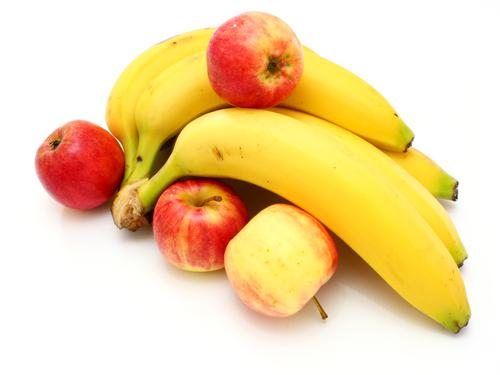
\includegraphics[scale=0.4]{banana}
  \end{center}

  \pause Bug reports (Apples) coming in.
  \pause \par Similar bug reports? What about tech articles (Bananas)?
  \pause \par Need it ASAP!

\end{frame}

\begin{frame}{Defect}
  \begin{center}
    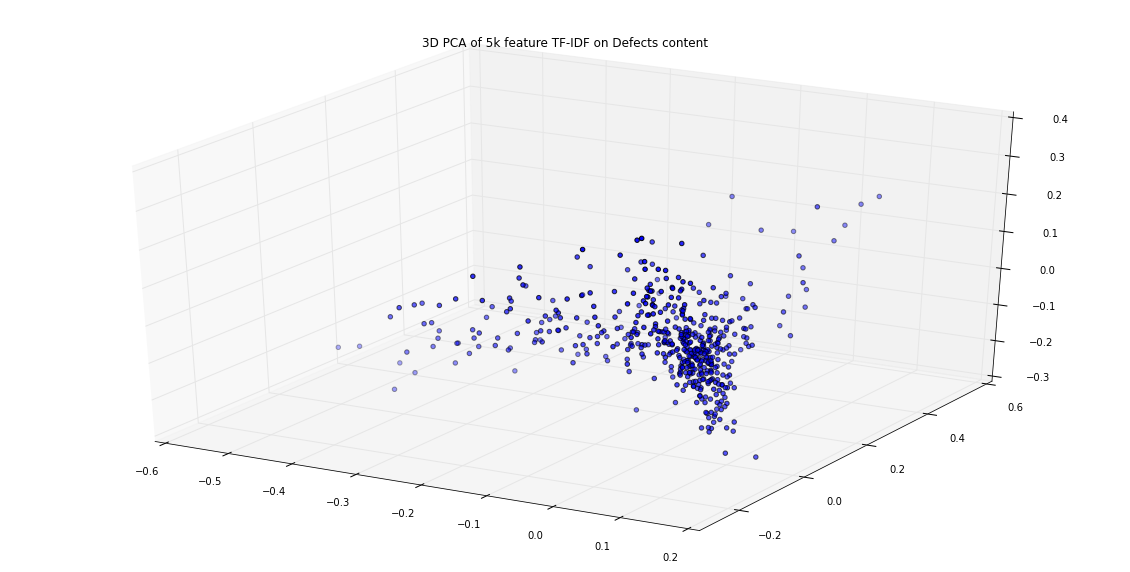
\includegraphics[scale=0.3]{tfidf_pca3d}
  \end{center}
\end{frame}

\begin{frame}
  \begin{center}
    Both have same structure: content $\rightarrow$ string similarity
      kernel (Lohdi, 2002)
     
    \pause 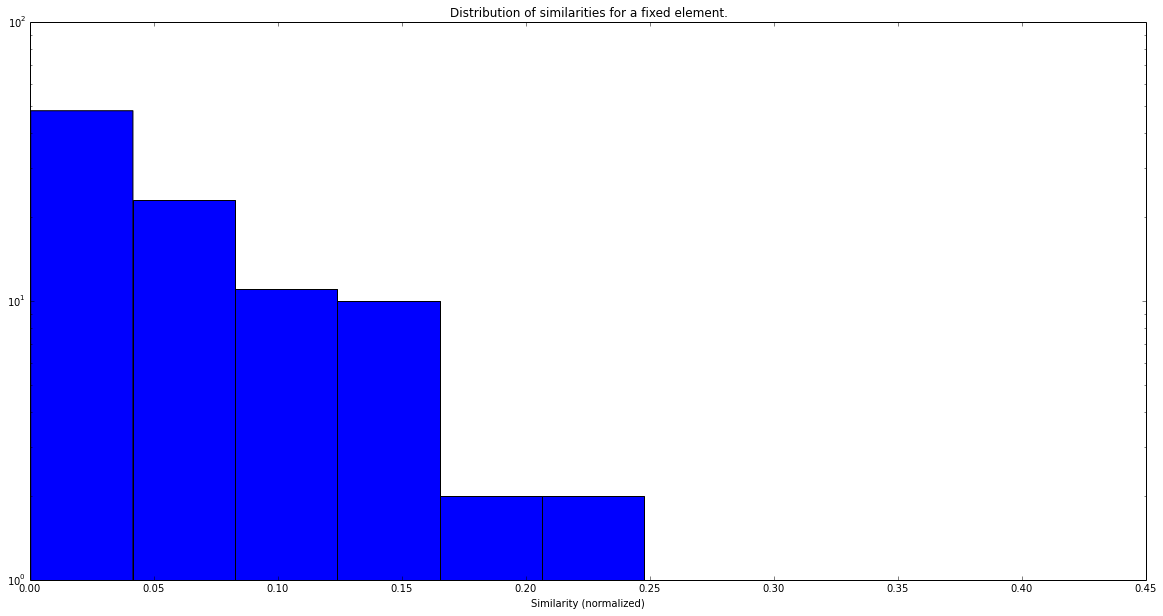
\includegraphics[scale=0.2]{kernel}
  \end{center}
\end{frame}

\begin{frame}[Pros]
    \begin{itemize}
      \item Model can incorporate more information (e.g. if both are apples,
        prior knowledge)
      \item Possible to use in an online setting (cf. online SVM)
      \item Free algorithms.
    \end{itemize}
\end{frame}

\begin{frame}[Cons]
  \begin{itemize}
    \item Slow to compute all pairwise similarities (be clever i.e. clustering)
    \item Kernel methods not really supported in Big Data.
  \end{itemize}
\end{frame}

\begin{frame}
  Thanks for your attention! \\ \\
  Questions?
\end{frame}

\end{document}
